\documentclass[11pt]{jsarticle}  % 文字の大きさは調整可能
%紙サイズ：A4(297mm×210mm)
%文字サイズ：11pt(調整可能)

\usepackage{zemistyle}
%\usepackage{amsmath}
%\usepackage{amsfonts}
%\usepackage{enumerate}
\usepackage{amssymb}
\usepackage{booktabs}
\usepackage{subcaption}
\usepackage{multirow}
\usepackage{newtxtext,newtxmath}%英数字書体として「Times new Roman」を使う
\usepackage[dvipdfmx]{graphicx}
\usepackage[hyphens]{url}

\setcounter{topnumber}{6}
\setcounter{bottomnumber}{5}
\setcounter{totalnumber}{11}
\setcounter{dbltopnumber}{5}
\renewcommand{\topfraction}{.999}
\renewcommand{\dbltopfraction}{.999}
\renewcommand{\bottomfraction}{.999}
\renewcommand{\textfraction}{.001}
\renewcommand{\floatpagefraction}{.999}
\renewcommand{\dblfloatpagefraction}{.999}
\renewcommand{\baselinestretch}{1.0} % 行間の調整
\newcommand{\Hline}{\noalign{\hrule height 0.4mm}}
\newcommand{\vect}[1]{\mbox{\boldmath$#1$}}
\newcommand{\svect}[1]{\mbox{\scriptsize\boldmath $#1$}}


\begin{document}
%%%%%%%%%%%%%%%%%%%%%%%%%%%%%%%%%%%%%%%%%%%%%%%%%%%%%%%%%%%%%%%%%%%%%%%%%%%%%%%%%%%%%%%%%%%%%%
% Title and author information
%%%%%%%%%%%%%%%%%%%%%%%%%%%%%%%%%%%%%%%%%%%%%%%%%%%%%%%%%%%%%%%%%%%%%%%%%%%%%%%%%%%%%%%%%%%%%%
\title{
サンプルタイトル
}

\date{\large \today}
\author{
  \large {学籍番号} ~ {指名}
}

\maketitle
%%%%%%%%%%%%%%%%%%%%%%%%%%%%%%%%%%%%%%%%%%%%%%%%%%%%%%%%%%%%%%%%%%%%%%%
% Beginning of the document
%%%%%%%%%%%%%%%%%%%%%%%%%%%%%%%%%%%%%%%%%%%%%%%%%%%%%%%%%%%%%%%%%%%
\section{はじめに}
\label{sec:intro}
これは文字の大きさ，行間等を確認するための文章です．自由に書き換えて使用してください．
これは文字の大きさ，行間等を確認するための文章です．自由に書き換えて使用してください．
これは文字の大きさ，行間等を確認するための文章です．自由に書き換えて使用してください．
これは文字の大きさ，行間等を確認するための文章です．自由に書き換えて使用してください．
これは文字の大きさ，行間等を確認するための文章です．自由に書き換えて使用してください．
これは文字の大きさ，行間等を確認するための文章です．自由に書き換えて使用してください．


%%%%%%%%%%%%%%%%%%%%%%%%%%%%%%%%%%%%%%%%%%%%%%%%%%%%%%%%%%%%%%%%%%%
\section{セクション1\cite{AAA}}
\label{sec:section1}
これは文字の大きさ，行間等を確認するための文章です．自由に書き換えて使用してください．
これは文字の大きさ，行間等を確認するための文章です．自由に書き換えて使用してください．
これは文字の大きさ，行間等を確認するための文章です．自由に書き換えて使用してください．
これは文字の大きさ，行間等を確認するための文章です．自由に書き換えて使用してください．


%%%%%%%%%%%%%%%%%%%%%%%%%%%%%%%%%%
\subsection{サブセクション1}
\label{sec:subsection1}
これは文字の大きさ，行間等を確認するための文章です．自由に書き換えて使用してください．
これは文字の大きさ，行間等を確認するための文章です．自由に書き換えて使用してください．
これは文字の大きさ，行間等を確認するための文章です．自由に書き換えて使用してください\cite{BBB}．
\begin{equation}
  \label{eq:dfm_loss}
  \mathcal{L}(\theta) = 
  \mathbb{E}_{t, X_t}
    \left[
      \sum_{i \in \{d\}}
        D_{X_t}\left(u_t^{(i)}(\cdot, X_t) , \hat{u_t}^{(i)}(\cdot, X_t; \theta)\right)
    \right]
\end{equation}
\ref{eq:dfm_loss}
これは文字の大きさ，行間等を確認するための文章です．自由に書き換えて使用してください．
これは文字の大きさ，行間等を確認するための文章です．自由に書き換えて使用してください．
これは文字の大きさ，行間等を確認するための文章です．自由に書き換えて使用してください．
\begin{align}
  \label{eq:ddm_cfg}
  &p_{\gamma, t+1 \mid \mathcal{C}, t}(x_{t+1} \mid c,x_{t}) \notag \\
  = &\prod_{i=1}^d
    \frac
      {p_{t+1 \mid \mathcal{C}, t}(x_{t+1}^{(i)} \mid c,x_{t})^\gamma
       p_{t+1 \mid t}(x_{t+1}^{(i)} \mid x_{t})^{1-\gamma}}
      {\sum_{x_{t+1}'} p_{t+1 \mid \mathcal{C}, t}(x_{t+1}' \mid c,x_{t})^\gamma
       p_{t+1 \mid t}(x_{t+1}' \mid x_{t})^{1-\gamma}} 
\end{align}


%%%%%%%%%%%%%%%%%%%%%%%%%%%%%%%%%%%%%%%%%%%%%%%%%%%%%%%%%%%%%%%%%%%


\section{セクション2}
これは文字の大きさ，行間等を確認するための文章です．自由に書き換えて使用してください．
これは文字の大きさ，行間等を確認するための文章です．自由に書き換えて使用してください．
これは文字の大きさ，行間等を確認するための文章です．自由に書き換えて使用してください．
これは文字の大きさ，行間等を確認するための文章です．自由に書き換えて使用してください．

\begin{figure}[h]
  \centering
  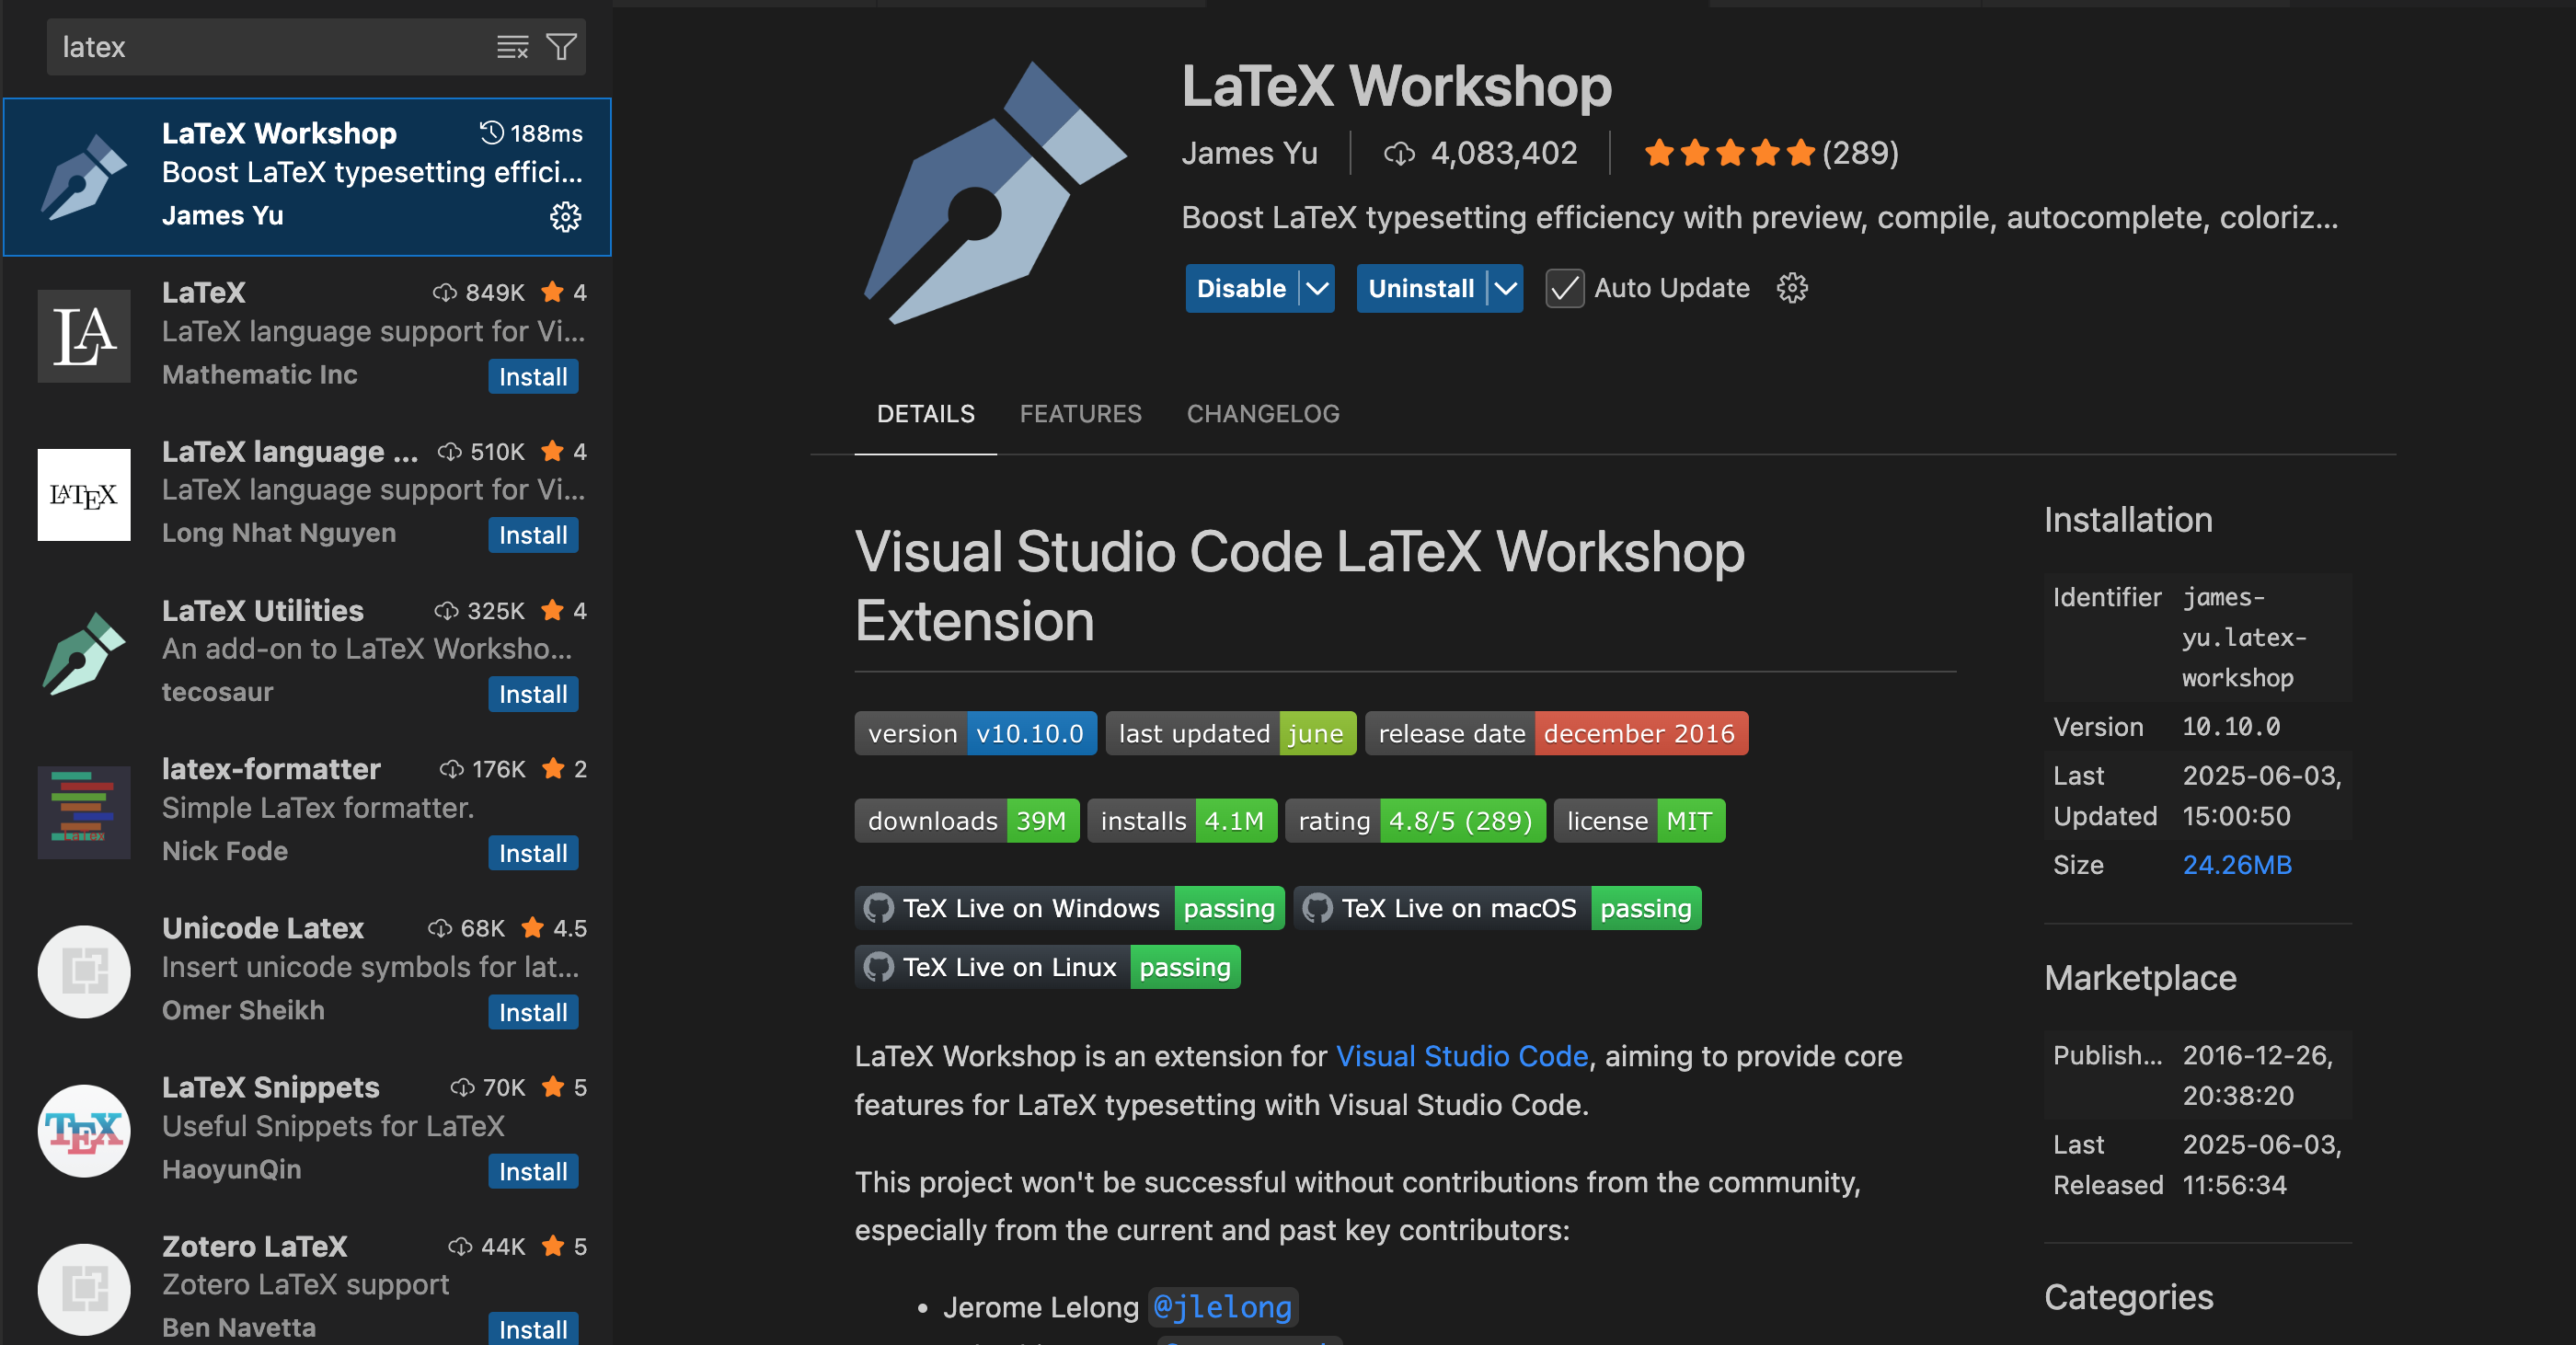
\includegraphics[width=0.6\linewidth]{figures/latex.png}  % 幅は画像に応じて調整
  \caption{テストキャプション}
  \label{fig:sample_caption}
\end{figure}

\ref{fig:sample_caption}
これは文字の大きさ，行間等を確認するための文章です．自由に書き換えて使用してください．
これは文字の大きさ，行間等を確認するための文章です．自由に書き換えて使用してください．

\begin{figure}[h]
  \centering
  \begin{minipage}[t]{0.48\linewidth}  % 幅を調整（0.48～0.49 が無難）
    \centering
    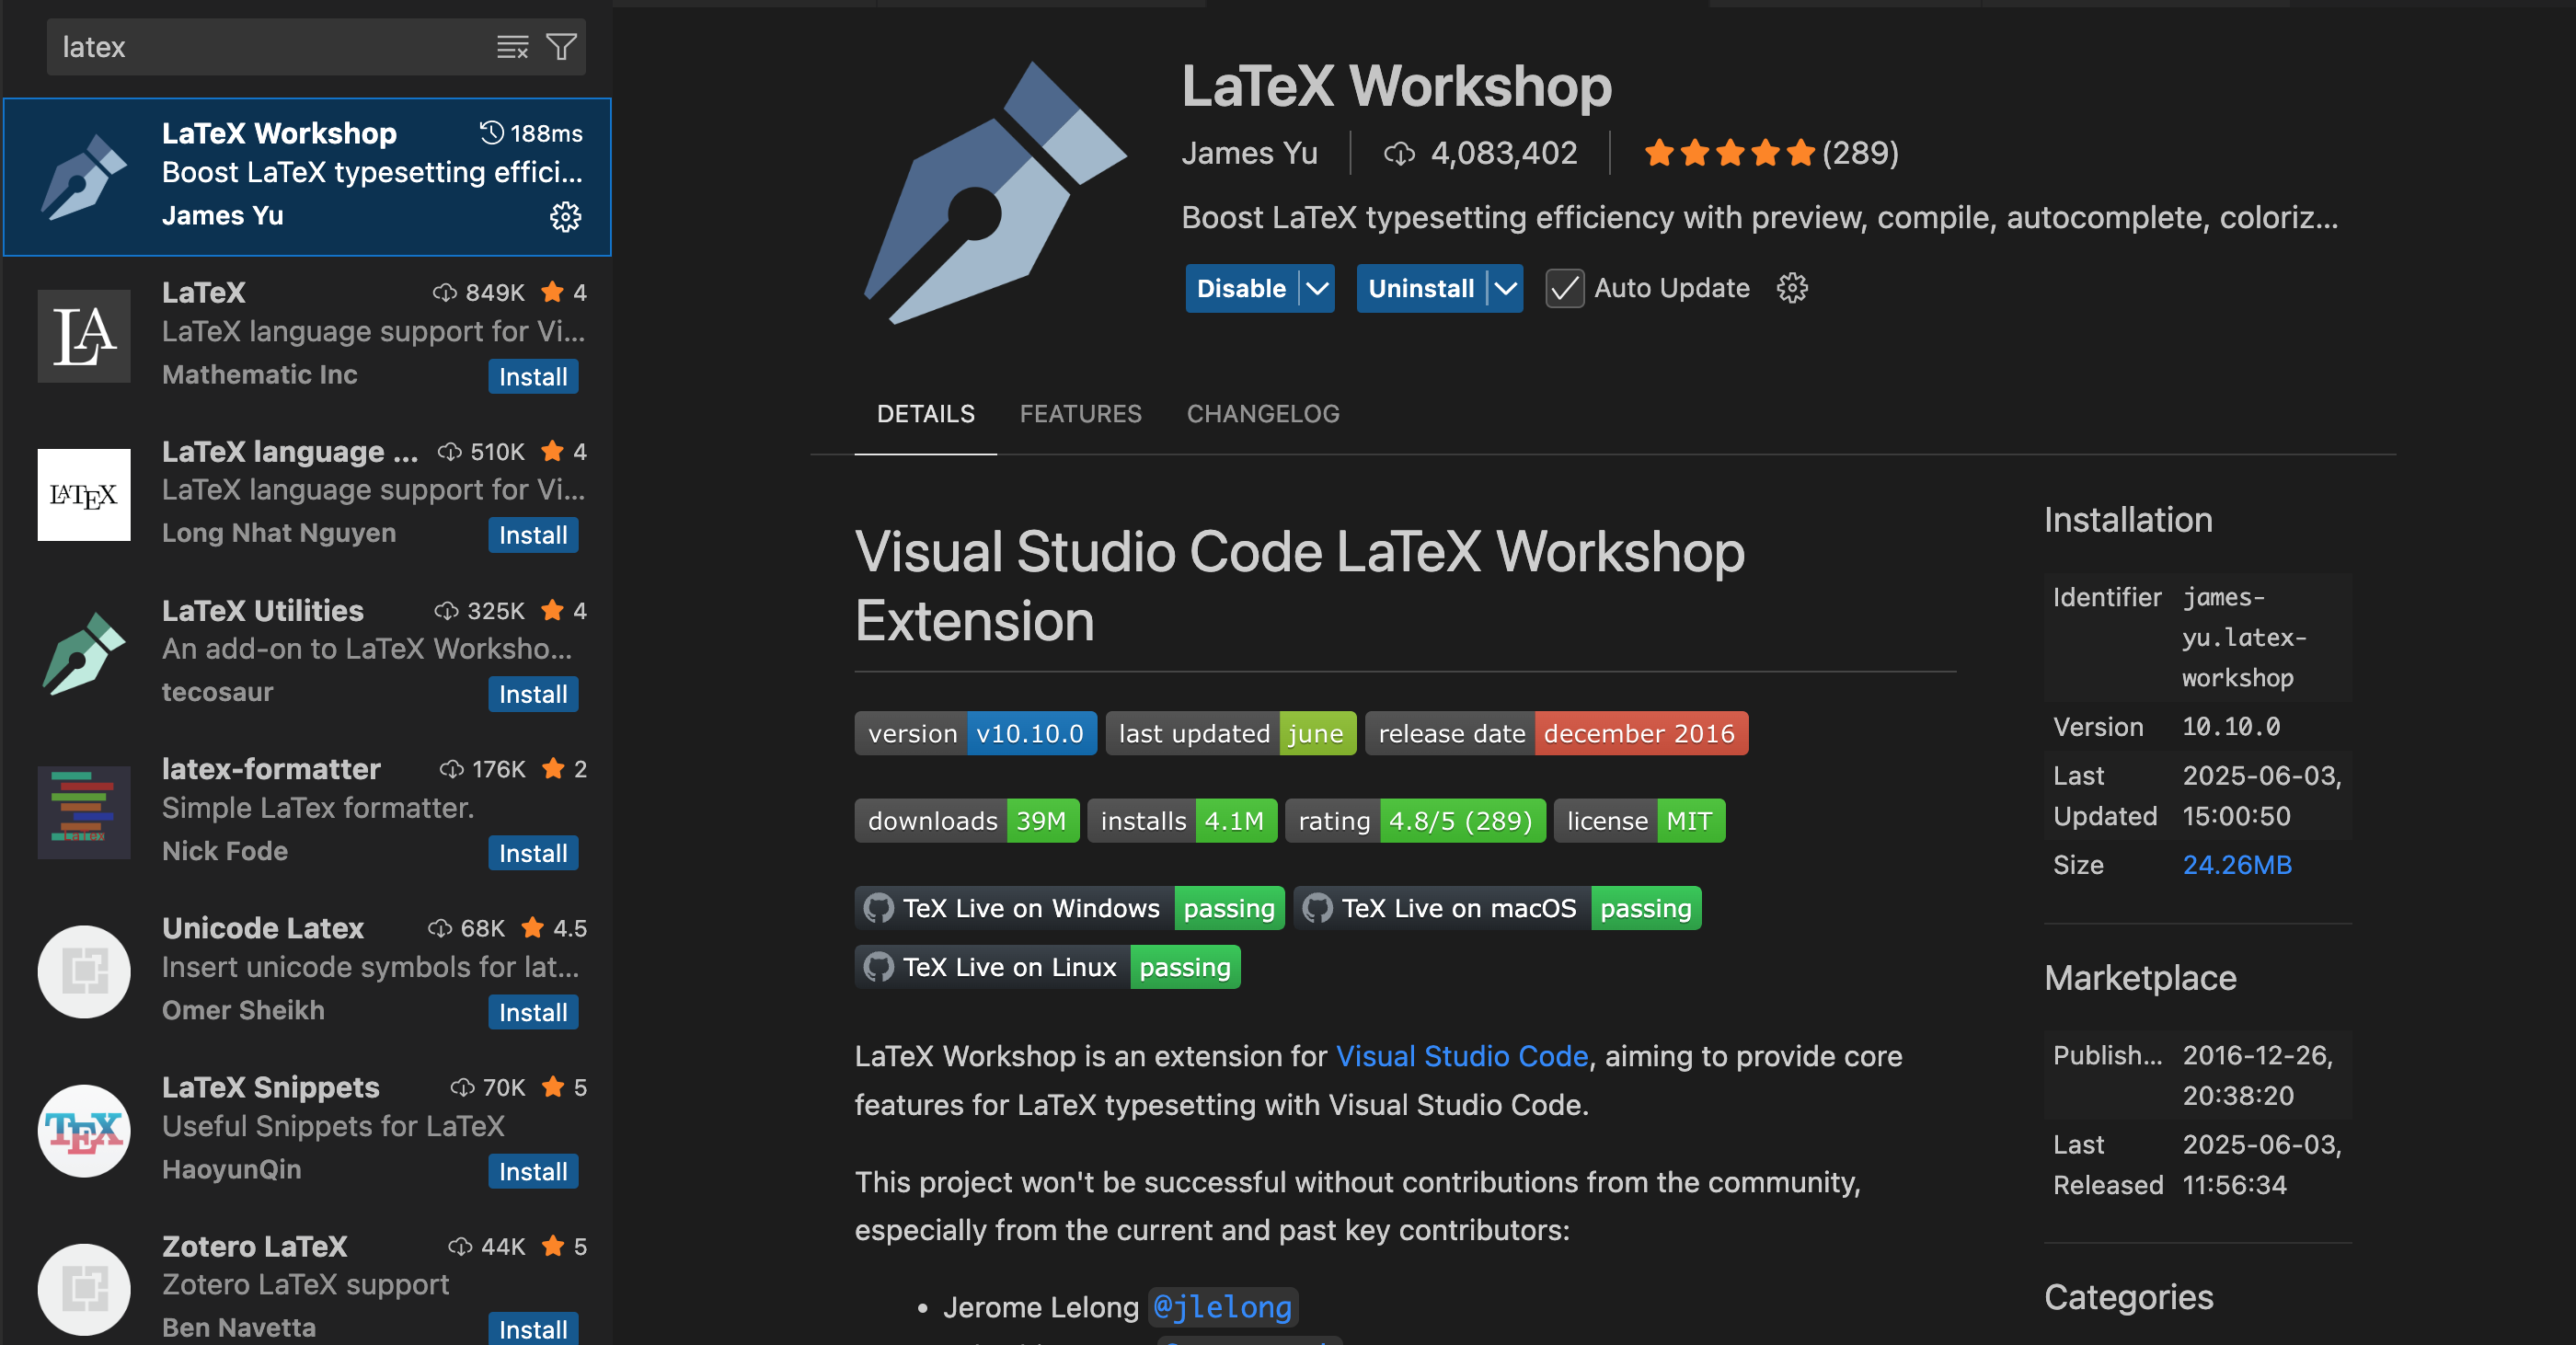
\includegraphics[width=\linewidth]{figures/latex.png}
    \caption{横並びの図1}
    \label{fig:sample_caption2}
  \end{minipage}
  \hfill  % 図間の水平スペース
  \begin{minipage}[t]{0.48\linewidth}
    \centering
    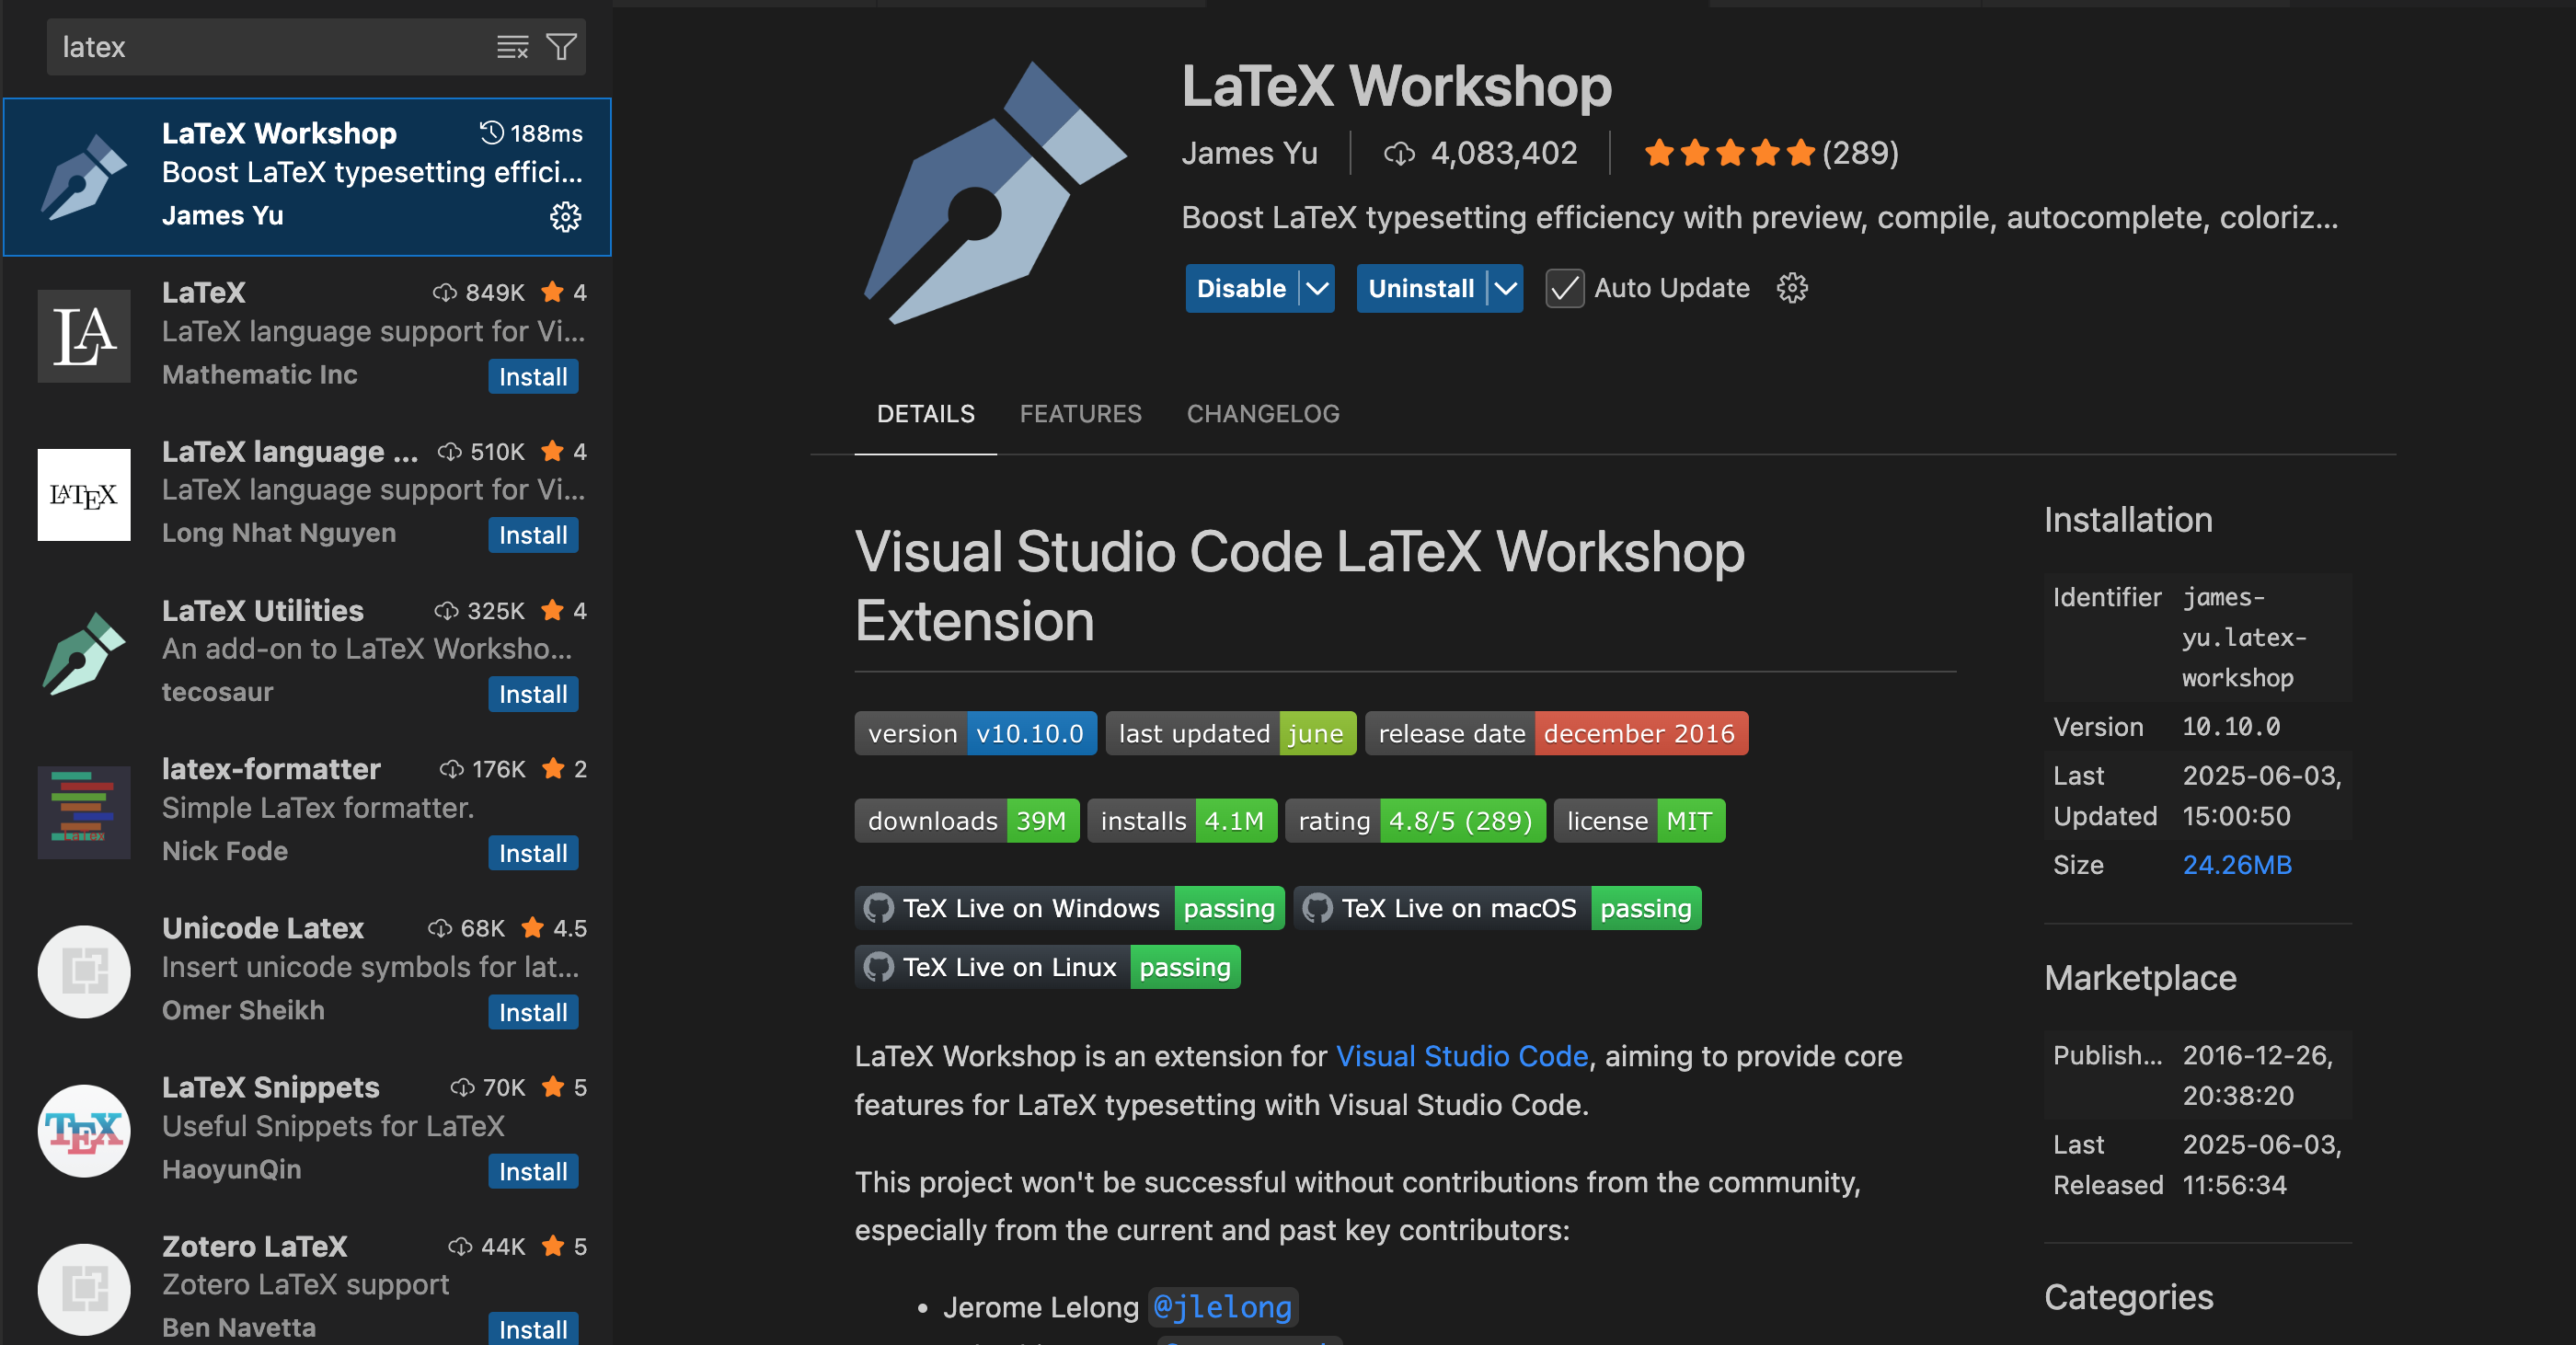
\includegraphics[width=\linewidth]{figures/latex.png}
    \caption{横並び図2}
    \label{fig:sample_caption3}
  \end{minipage}
\end{figure}

これは文字の大きさ，行間等を確認するための文章です．自由に書き換えて使用してください．
これは文字の大きさ，行間等を確認するための文章です．自由に書き換えて使用してください．


%%%%%%%%%%%%%%%%%%%%%%%%%%%%%%%%%%%%%%%%%%%%%%%%%%%%%%%%%%%%%%%%%%%%%%%%%%%%%%%%%%%%%%%%
\section{おわりに}
これは文字の大きさ，行間等を確認するための文章です．自由に書き換えて使用してください．
これは文字の大きさ，行間等を確認するための文章です．自由に書き換えて使用してください．


\vspace{8ex}

%%%%%%%%%%%%%%%%%%%%%%%%%%%%%%%%%%%%%%%%%%%%%%%%%%%%%%%%%%%%%%%%%%%%%%%%%%%%%%%%%%%%%%%%
%\renewcommand{\baselinestretch}{0.9}
\newpage
\begin{thebibliography}{99}
\setlength{\itemsep}{1.5pt}
% \small % 必要に応じて

\bibitem{AAA}
M. Fujioka, M. Fujioka, and M. Fujioka,
``A Sample Paper for Zemi Style,''
Proc.\ 99th Conf.\ on Sample Conference Name (SCN 2024),
pp. 1--10,
Jun.~2025.


\bibitem{BBB}
M. Fujioka, M. Fujioka, and M. Fujioka,
``A Sample Paper for Zemi Style,''
Proc.\ 99th Conf.\ on Sample Conference Name (SCN 2024),
pp. 1--10,
Jun.~2025.

\end{thebibliography}

\end{document}